\section{Indspænding} \label{Indspænding}

Til indspændingen gøres der brug af indspændingselementer og en stål plade, med jævnt fordelte huller langs siderne. Pladen har til formål at bære emnet, samt bære indspændingselementerne. Bundpladen er en \SI{6}{mm} tyk rustfri AISI 304 stålplade \parencite{Stalet2025KbMal}.

Rustfri AISI 304 stål er et materiale med væsentligt højere densitet, omkring \SI{7900}{kg/m^3}, og en E-modul på cirka \SI{193}{GPa}. Stål tilbyder en betydeligt højere stivhed og styrke end aluminium, hvilket gør det særlig egnet til komponenter, som udsættes for store belastninger eller gentagen mekanisk påvirkning. flydespænding for almindelige konstruktionsstål ligger typisk omkring \SI{215}{MPa}, mens trækstyrken ligger mellem \SI{500}{MPa} og \SI{750}{MPa}. Denne høje styrke gør stål velegnet til områder, hvor strukturel integritet og dimensionsstabilitet er afgørende over lang tid. Stål tillader nøjagtig maskinbearbejdning og tilbyder robuste svejseegenskaber, hvilket kan være en fordel i konstruktioner, hvor stor præcision og høj samlingsstyrke er påkrævet. Til bundplanden vælges AISI 304 stål for dets rustfri egenskaber, fordi det vurderes sandsynligt, at farvemidler kan komme på bundpladen. Prisen på stål ligger relativt lavt i forhold til andre materialer, med en gennemsnitlig pris på omkring 79 DKK pr. kg \parencite{Stalprofil}, hvilket gør det attraktivt i applikationer, hvor vægt ikke er den primære begrænsning \parencite{Jessen2011RustfritKorrosion}.


Der bores 32 \SI{10}{mm} huller, syv på hver af de to lang sider og ni på hver af kort siderne. De 32 huller er til placering af indspænding elementerne, hvor 24 af dem er placeret uden for arbejdes området og de resterende otte er placeret inde i arbejdets området på de korte sider. Yderligere bores der et M6 hul i hvert hjørne, som skal tillade at pladen kan fastspændes til stellet med fire M6 bolte. se figur \ref{fig: bundplade}


\begin{figure}[H]
    \centering
    \begin{subfigure}[b]{0.49\textwidth}
         \centering
        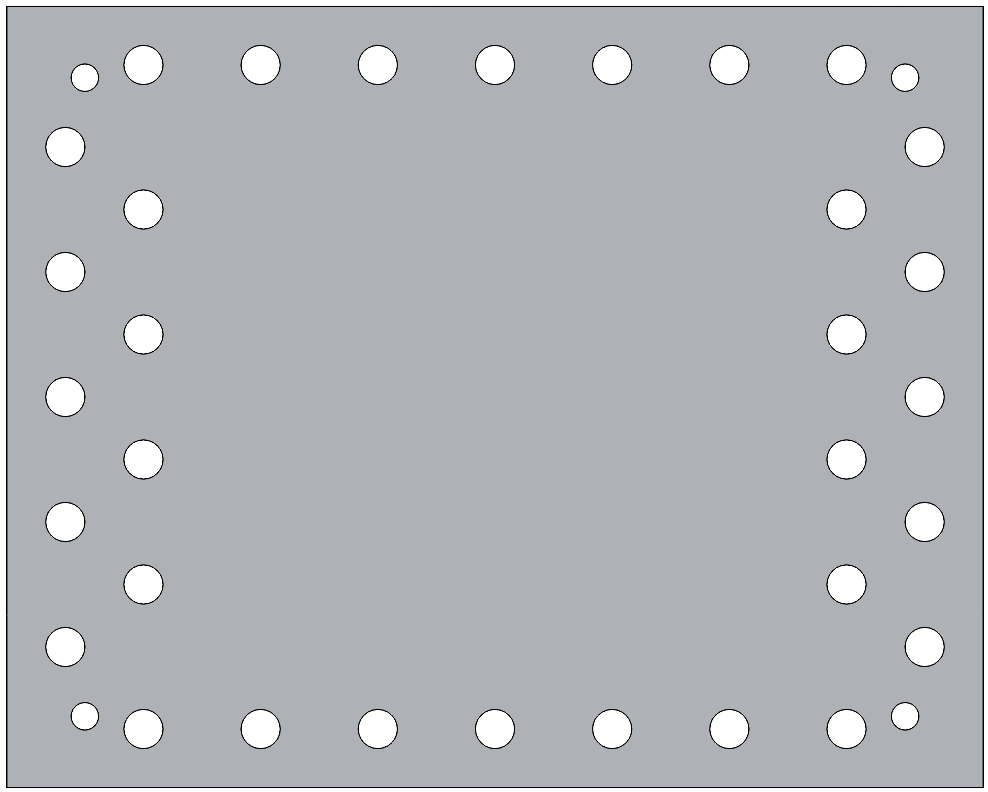
\includegraphics[width=.8\linewidth]{Sections/6 Detaljeløsning/Media/bundplade.png}
         \caption{Illustration af bundplade set oppe fra.}
       \label{fig: bundplade}
    \end{subfigure}
    \begin{subfigure}[b]{0.49\textwidth}
      \centering
      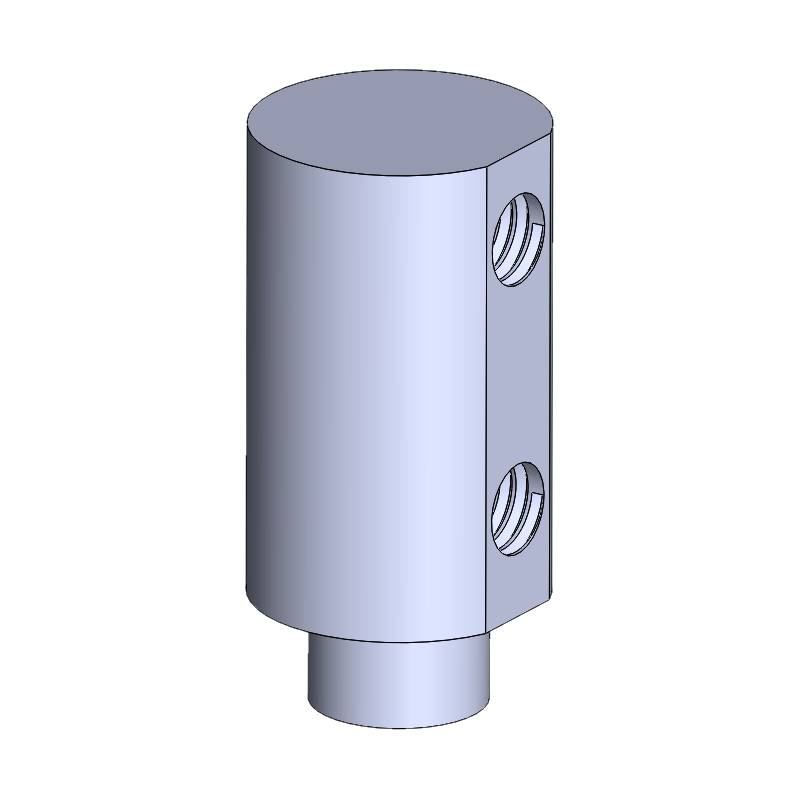
\includegraphics[width=.7\linewidth]{Sections/6 Detaljeløsning/Media/Billeder til indspænding/Gevindholder.png}
      \caption{Gevindholder.}
      \label{fig: gevindholder}
    \end{subfigure}
    \caption{Dele til indspædning}
\end{figure} \plainbreak{-.5}

Indspændingselementer er delene der indspænder emnet. De består af tre dele: en gevindholder (figur \ref{fig: gevindholder}), en \SI{100}{mm} M6 bolt med en gevindhældning på \SI{1}{mm} \parencite{RSComponents2025M6RS} og en PVC endeprop \parencite{Profillageret2025RundProfillageret.dk}. Gevindholderne placeres i et af pladens \SI{10}{mm} huller. De \SI{100}{mm} lange M6 bolte køre igennem gevindholderne, som gør at boltene gradvist spændes mod emnet. For at undgå at emnet beskadiges under indspændingen, er der monteret endeprop på boltenes ende der har kontakt med emnet.

% Skrive om hvor vi har valgt et frirum 3mm. Det med at bolten skal kunne dreje uden problemer.
% To huller for frihed
% Valg for at gøre den rund. Kom ind på optimale fremstilling, samt man kan dreje den så den passer til emener der har skæve former.


For at tage højde for forskellige emne højder, er gevindholderen udforment med to gevind huller, hvilket betyder der kan vælges mellem de to huller alt efter emne højde. Det nederste hul har en fri højde fra pladen på \SI{3}{mm}, for at sikre at bolten ikke kommer i kontakt med pladen, under indspænding. Derudover er frihøjden også valgt ud fra bolten ikke skal være besværlig for forbrugen at tilgå.
Gevindholderens runde form er valgt på baggrund af henholdvis fremstillingsårsager, samt en evne til at kunne passe til emner med skræve former. Ved emner hvor dets sider ikke ligger parallelt med pladens sider, muliggøre gevind holderens cylindriske form, at den kan vinkles til at give den mest optimale kontaktflade med emnet.


Til produktet medfølger seks indspændings elementer, hvortil to af dem er tiltænkt som reserve, eller til tilfælde med ikke prismatiske emner. Det er derved tiltænkt at emner indspændes med to indspændingselementer, som vist på figur \ref{fig: indspænding}. 

\begin{figure}[H]
    \centering
    \begin{subfigure}[b]{0.48\textwidth}
    \centering
         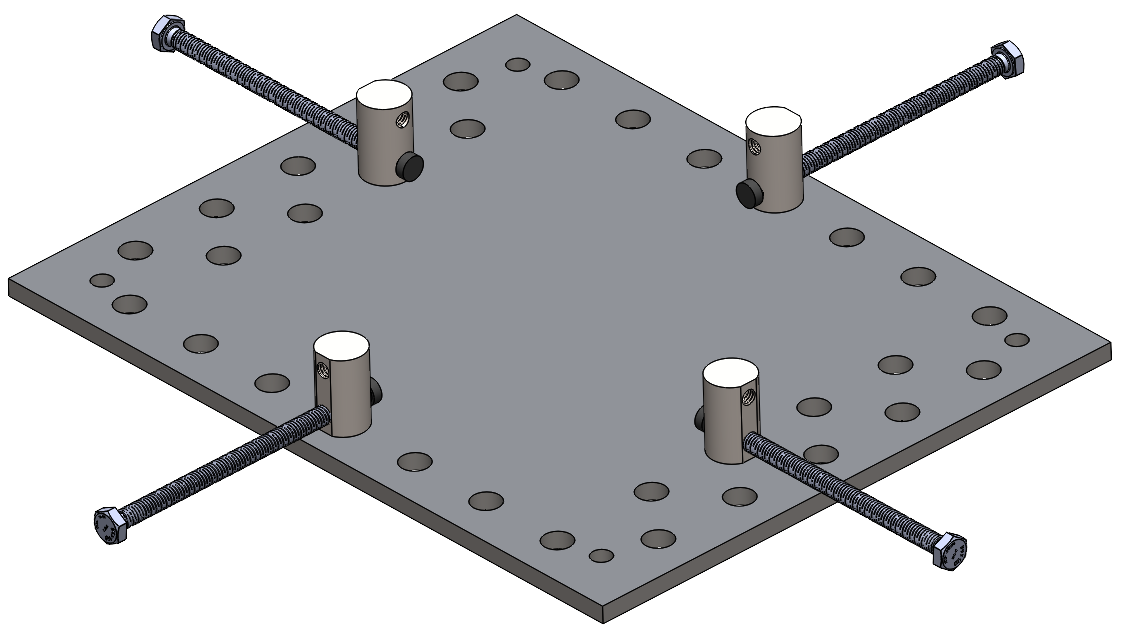
\includegraphics[width=0.9\linewidth]{Sections/6 Detaljeløsning/Media/Indspænding lav.png}
     \caption{Laveste position}
      \label{fig: indspænding lav}
    \end{subfigure} 
    \begin{subfigure}[b]{0.48\textwidth}
    \centering
        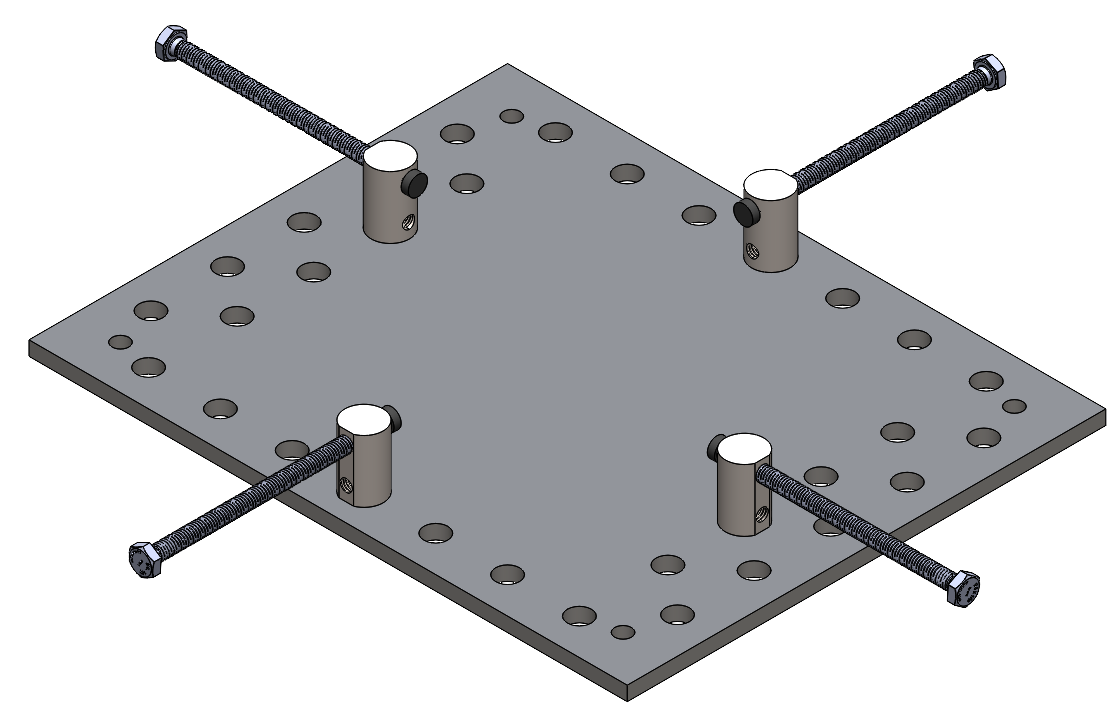
\includegraphics[width=0.9\linewidth]{Sections/6 Detaljeløsning/Media/Indspænding høj.png}
     \caption{Højeste position}
      \label{fig: indspænding høj}
    \end{subfigure}
    \caption{Opstilling af indspændingen hvor bolten er i henholdsvis den laveste og højeste position. Arbejdstegninger kan ses i bilag \ref{Bilag - arbejdstegniner}}
    \label{fig: indspænding}
\end{figure} \plainbreak{-.5}

Bundpladen er $\SI{270}{mm} \times \SI{220}{mm} \times \SI{6}{mm}$, og har en volumen på  $ 340,4 \cdot 10^{-9} \SI{}{m^3}$ der med en densitet på $\approx \SI{7900}{kg \cdot m^{-3}}$ giver en vægt på $\approx \SI{2,8}{kg}$. 